%===============================================================================
\chapter{Algebraic Foundations of Renormalization}
\label{ch:algebra}
%===============================================================================

\marginnote{This chapter reveals the deep algebraic structure underlying renormalization, starting with its origins in the numerical analysis of ODEs before showing how the same structure appears in quantum field theory.}

The preceding chapters developed the practical machinery for perturbation theory, and we have seen perturbative expansions fail in various ways. This chapter reveals the deeper algebraic structure that organizes these expansions and their renormalization. The remarkable fact is that the same algebraic structure appears in two seemingly unrelated contexts, namely ordinary differential equations and quantum field theory.

\begin{itemize}
\item \textbf{Section~\ref{sec:butcher}}: The Butcher group and B-series for ODEs, where rooted trees organize perturbative solutions
\item \textbf{Section~\ref{sec:hopf_algebra}}: The Hopf algebra of Feynman graphs, showing the same structure in QFT
\item \textbf{Section~\ref{sec:riemann_hilbert}}: The Riemann-Hilbert correspondence, connecting renormalization to complex analysis through the Birkhoff decomposition
\item \textbf{Section~\ref{sec:hopf_resurgence}}: Connection to resurgent structure, showing how the algebraic picture complements the analytic one
\end{itemize}

The key insight is that renormalization is not an ad hoc procedure for canceling infinities. Rather, it is a mathematically natural operation with deep algebraic structure. This structure was first discovered by Butcher (1963) in the context of numerical methods for ODEs, and was later recognized by Connes and Kreimer (1998--2000) to be the same structure governing renormalization in quantum field theory.

\marginnote{Connes and Kreimer (1999) wrote of Butcher's work on numerical integration methods as ``an impressive example that concrete problem-oriented work can lead to far-reaching conceptual results.''}

%-------------------------------------------------------------------------------
\section{The Butcher Group: Hopf Algebras from ODEs}
\label{sec:butcher}
%-------------------------------------------------------------------------------

Before encountering Hopf algebras in quantum field theory, we develop the same structures in a simpler setting: ordinary differential equations. This is not merely pedagogy. Historically, the Hopf algebra of rooted trees arose first in numerical analysis, and Connes--Kreimer recognized that the Hopf algebra of Feynman graphs is essentially the same object.

\marginnote{John C. Butcher introduced the algebraic theory of Runge--Kutta methods in 1963. The infinite-dimensional Lie group of characters was identified by Hairer and Wanner (1974) and is now called the \textbf{Butcher group}.}

\subsection{Rooted Trees and Elementary Differentials}
\label{sec:rooted_trees}

Consider the autonomous ODE
\begin{equation}
\frac{dx}{ds} = f(x), \qquad x(0) = x_0
\label{eq:autonomous_ode}
\end{equation}
where $x \in \mathbb{R}^N$ and $f: \mathbb{R}^N \to \mathbb{R}^N$ is smooth. We seek a formal power series solution in time $s$. The key observation, going back to Cayley (1857), is that the higher derivatives of $x(s)$ are naturally indexed by \textbf{rooted trees}.

\begin{definition}[Rooted Tree]
A \textbf{rooted tree} is a connected graph with no cycles and a distinguished node called the \textbf{root}. The number of nodes in a tree $t$ is denoted $|t|$.
\end{definition}

The first few rooted trees, organized by number of nodes, are shown below. We denote the single-node tree (just a root) by $\bullet$.

\begin{center}
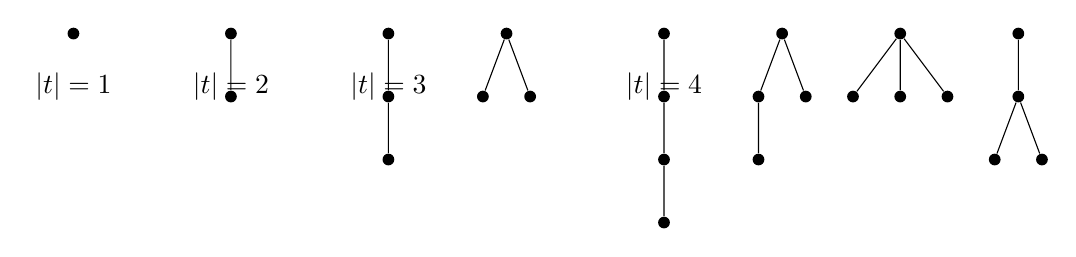
\begin{tikzpicture}[
    level distance=8mm,
    sibling distance=6mm,
    every node/.style={circle,fill,inner sep=1.5pt}
]
% n=1
\node[label=below:{$|t|=1$}] at (0,0) {};

% n=2
\node[label=below:{$|t|=2$}] at (2,0) {}
  child {node {}};

% n=3: two trees
\node[label=below:{$|t|=3$}] at (4,0) {}
  child {node {}
    child {node {}}
  };
\node at (5.5,0) {}
  child {node {}}
  child {node {}};

% n=4: four trees  
\node[label=below:{$|t|=4$}] at (7.5,0) {}
  child {node {}
    child {node {}
      child {node {}}
    }
  };
\node at (9,0) {}
  child {node {}
    child {node {}}
  }
  child {node {}};
\node at (10.5,0) {}
  child {node {}}
  child {node {}}
  child {node {}};
\node at (12,0) {}
  child {node {}
    child {node {}}
    child {node {}}
  };
\end{tikzpicture}
\end{center}

\marginnote{There are 1, 1, 2, 4, 9, 20, 48, 115, \ldots rooted trees with $n = 1, 2, 3, 4, 5, 6, 7, 8, \ldots$ nodes. This is OEIS sequence A000081.}

Given a tree $t = [t_1, t_2, \ldots, t_k]$ formed by attaching the roots of subtrees $t_1, \ldots, t_k$ to a new common root, we define the \textbf{elementary differential} $\delta_t(x)$ recursively.

\begin{definition}[Elementary Differential]
For a vector field $f: \mathbb{R}^N \to \mathbb{R}^N$, define the elementary differentials by
\begin{align}
\delta_\bullet^i(x) &= f^i(x) \\
\delta_{[t_1, \ldots, t_k]}^i(x) &= \sum_{j_1, \ldots, j_k = 1}^N \left(\delta_{t_1}^{j_1}(x) \cdots \delta_{t_k}^{j_k}(x)\right) \frac{\partial^k f^i}{\partial x^{j_1} \cdots \partial x^{j_k}}(x)
\end{align}
\end{definition}

\textbf{Physical interpretation:} Each rooted tree encodes a specific pattern of nested differentiations. The root corresponds to the outermost function $f$, and each subtree corresponds to differentiation with respect to one argument, followed by substitution of another instance of $f$. This structure captures exactly the chain rule applied repeatedly.

\begin{workedbox}[Box 7.1: Elementary Differentials for Small Trees]
\textbf{Goal:} Compute the elementary differentials for trees with up to 3 nodes.

\textbf{The single-node tree $\bullet$:}
\begin{equation}
\delta_\bullet = f
\end{equation}
This is just the vector field itself.

\textbf{The two-node tree $[\bullet]$:}
\begin{equation}
\delta_{[\bullet]}^i = \sum_j f^j \frac{\partial f^i}{\partial x^j} = (f \cdot \nabla) f^i = (Df) \cdot f
\end{equation}
This is the directional derivative of $f$ along $f$, representing $\ddot{x} = \frac{d^2 x}{ds^2}$.

\textbf{The three-node chain $[[\bullet]]$:}
\begin{equation}
\delta_{[[\bullet]]}^i = \sum_{j,k} f^k \frac{\partial f^j}{\partial x^k} \frac{\partial f^i}{\partial x^j} + \sum_{j,k} f^j f^k \frac{\partial^2 f^i}{\partial x^j \partial x^k}
\end{equation}
This corresponds to $\dddot{x}$ computed via repeated application of the chain rule.

\textbf{The three-node ``fork'' $[\bullet, \bullet]$:}
\begin{equation}
\delta_{[\bullet,\bullet]}^i = \sum_{j,k} f^j f^k \frac{\partial^2 f^i}{\partial x^j \partial x^k}
\end{equation}
This is the second derivative of $f$ contracted with two copies of $f$.

\textbf{Key insight:} Different trees at the same order correspond to different ways of differentiating $f$. The tree structure keeps track of the combinatorics automatically.
\end{workedbox}

\subsection{B-Series: Formal Solutions Indexed by Trees}
\label{sec:bseries}

The remarkable fact is that the Taylor series solution of~\eqref{eq:autonomous_ode} can be written as a sum over rooted trees.

\begin{theorem}[B-Series Expansion]
The formal solution of $\dot{x} = f(x)$, $x(0) = x_0$ is
\begin{equation}
x(s) = x_0 + \sum_{\text{trees } t} \frac{s^{|t|}}{\sigma(t)} \delta_t(x_0)
\label{eq:bseries}
\end{equation}
where the sum runs over all rooted trees $t$, and $\sigma(t)$ is the \textbf{symmetry factor} of the tree (the order of its automorphism group times the tree factorial).
\end{theorem}

\marginnote{The symmetry factor $\sigma(t)$ accounts for equivalent ways of building the same tree. It is analogous to the symmetry factors of Feynman diagrams.}

The B-series (``Butcher series'') provides a universal framework for analyzing:
\begin{itemize}
\item The exact flow of a vector field (expanding the exponential map)
\item Runge--Kutta and other numerical integration methods
\item Composition of flows and near-identity transformations
\end{itemize}

\textbf{Connection to the Prologue:} The perturbative solution of the damped anharmonic oscillator from the Prologue can be written as a B-series. Each tree corresponds to a specific pattern of interactions between the linear and nonlinear parts of the vector field. Secular terms arise when certain tree contributions grow unboundedly in time.

\subsection{The Hopf Algebra of Rooted Trees}
\label{sec:hopf_trees}

The set of rooted trees carries a natural \textbf{Hopf algebra} structure. This structure organizes the composition and decomposition of flows.

\marginnote{A Hopf algebra is an algebra with a compatible coalgebra structure (coproduct, counit) and an antipode. It generalizes the notion of a group algebra.}

\begin{definition}[Hopf Algebra $\mathcal{H}_R$ of Rooted Trees]
Let $\mathcal{H}_R$ be the polynomial algebra over $\mathbb{C}$ generated by rooted trees, with the following structures.

\textbf{Product:} The product is the disjoint union of trees (forming a forest):
\begin{equation}
t_1 \cdot t_2 = t_1 \sqcup t_2
\end{equation}
The unit is the empty forest $\mathbf{1}$.

\textbf{Coproduct:} The coproduct $\Delta: \mathcal{H}_R \to \mathcal{H}_R \otimes \mathcal{H}_R$ encodes how trees can be ``cut'':
\begin{equation}
\Delta(t) = t \otimes \mathbf{1} + \mathbf{1} \otimes t + \sum_{\text{admissible cuts } c} P^c(t) \otimes R^c(t)
\label{eq:tree_coproduct}
\end{equation}
where $P^c(t)$ is the ``pruned'' part (subtrees removed by the cut) and $R^c(t)$ is the ``remainder'' (what remains attached to the root).

\textbf{Counit:} $\varepsilon(t) = 0$ for any non-empty tree, $\varepsilon(\mathbf{1}) = 1$.

\textbf{Antipode:} Defined recursively by
\begin{equation}
S(t) = -t - \sum_{\text{cuts } c} S(P^c(t)) \cdot R^c(t)
\label{eq:tree_antipode}
\end{equation}
\end{definition}

\begin{workedbox}[Box 7.2: The Coproduct for Small Trees]
\textbf{Goal:} Compute the coproduct for trees with 1, 2, and 3 nodes.

\textbf{Single node $\bullet$:} No non-trivial cuts are possible.
\begin{equation}
\Delta(\bullet) = \bullet \otimes \mathbf{1} + \mathbf{1} \otimes \bullet
\end{equation}
This says $\bullet$ is \textbf{primitive} (no internal structure to decompose).

\textbf{Two nodes $[\bullet]$:} One cut is possible, separating the root from its child.
\begin{equation}
\Delta([\bullet]) = [\bullet] \otimes \mathbf{1} + \mathbf{1} \otimes [\bullet] + \bullet \otimes \bullet
\end{equation}
The third term represents cutting the edge: the pruned part is $\bullet$ and the remainder is $\bullet$.

\textbf{Three-node chain $[[\bullet]]$:} Two cuts are possible.
\begin{equation}
\Delta([[\bullet]]) = [[\bullet]] \otimes \mathbf{1} + \mathbf{1} \otimes [[\bullet]] + \bullet \otimes [\bullet] + [\bullet] \otimes \bullet + \bullet \cdot \bullet \otimes \bullet
\end{equation}
The terms correspond to: no cut, full cut, cutting the top edge, cutting the bottom edge, and cutting both edges.

\textbf{Physical meaning:} The coproduct encodes how a complicated operation (flow to time $s+t$) decomposes into simpler operations (flow to time $s$, then flow to time $t$). Each cut corresponds to a way of factoring the computation.
\end{workedbox}

\subsection{The Butcher Group}
\label{sec:butcher_group}

The \textbf{Butcher group} $G$ is the group of characters of the Hopf algebra $\mathcal{H}_R$. A \textbf{character} is an algebra homomorphism $\phi: \mathcal{H}_R \to \mathbb{C}$ (or more generally into any commutative algebra $A$).

\marginnote{The Butcher group is an infinite-dimensional Lie group. Its Lie algebra consists of infinitesimal characters, which are derivations of the Hopf algebra.}

\textbf{Group structure:} Characters form a group under the \textbf{convolution product}:
\begin{equation}
(\phi_1 \star \phi_2)(t) = m \circ (\phi_1 \otimes \phi_2) \circ \Delta(t)
\end{equation}
where $m$ is multiplication in the target algebra.

\begin{itemize}
\item \textbf{Identity:} The counit $\varepsilon$
\item \textbf{Inverse:} $\phi^{-1} = \phi \circ S$ (composition with the antipode)
\end{itemize}

\textbf{Physical interpretation:} 
\begin{itemize}
\item Each character $\phi$ assigns numerical values to trees, specifying a particular flow or numerical method.
\item The convolution product corresponds to \textbf{composition of flows}.
\item The inverse corresponds to \textbf{time reversal} or \textbf{undoing a transformation}.
\end{itemize}

\subsection{Renormalization in the ODE Context}
\label{sec:ode_renorm}

The B-series solution~\eqref{eq:bseries} may contain \textbf{secular terms} that grow without bound, invalidating the perturbative expansion. This is the ODE analog of UV divergences in QFT.

\textbf{The renormalization procedure:} Just as in QFT, we absorb the problematic terms into redefined parameters (initial conditions, frequencies, amplitudes). In Hopf-algebraic terms:

\begin{enumerate}
\item The ``bare'' solution is a character $\phi_{\text{bare}}: \mathcal{H}_R \to A$ where $A$ contains the secular terms.
\item The ``renormalized'' solution is obtained by Birkhoff-type factorization: $\phi_{\text{bare}} = \phi_-^{-1} \star \phi_+$
\item The counterterms are encoded in $\phi_-^{-1}$; the finite answer is $\phi_+$.
\end{enumerate}

\marginnote{This is exactly the Goldenfeld--Oono RG procedure from the Prologue, now understood as Birkhoff factorization in the Butcher group.}

\begin{workedbox}[Box 7.3: The Anharmonic Oscillator in B-Series Language]
\textbf{Goal:} Connect the Prologue's anharmonic oscillator to the Hopf algebra framework.

\textbf{Setup:} The damped anharmonic oscillator $\ddot{x} + 2\gamma\dot{x} + \omega_0^2 x + \epsilon x^3 = 0$ can be written as a first-order system:
\begin{equation}
\frac{d}{dt}\begin{pmatrix} x \\ v \end{pmatrix} = \begin{pmatrix} v \\ -2\gamma v - \omega_0^2 x - \epsilon x^3 \end{pmatrix} = f_0 + \epsilon f_1
\end{equation}
where $f_0$ is the linear part and $f_1$ contains the cubic nonlinearity.

\textbf{B-series expansion:} The perturbative solution has the form
\begin{equation}
\begin{pmatrix} x(t) \\ v(t) \end{pmatrix} = \sum_{\text{trees } t} \frac{t^{|t|}}{\sigma(t)} a(t, \epsilon) \delta_t(x_0, v_0)
\end{equation}
where each tree is decorated to indicate whether vertices correspond to $f_0$ or $f_1$.

\textbf{Secular terms:} Trees containing certain patterns (repeated $f_0$ insertions at resonant frequencies) produce elementary differentials that grow as $t \cdot \cos(\omega_0 t)$ rather than staying bounded. These are the secular terms.

\textbf{The coproduct and counterterms:} The coproduct of a ``secular tree'' $t_{\text{sec}}$ contains terms of the form $t_{\text{sub}} \otimes t_{\text{rem}}$ where $t_{\text{sub}}$ is the problematic subtree. The RG procedure corresponds to:
\begin{enumerate}
\item Identifying secular subtrees (via the coproduct)
\item Computing counterterms (via the antipode)
\item Factoring into $\phi_-^{-1} \star \phi_+$ (Birkhoff decomposition)
\end{enumerate}

\textbf{Result:} The renormalized solution is the running amplitude and phase derived in the Prologue, now understood as the ``$\phi_+$'' part of a Birkhoff factorization in the Butcher group.
\end{workedbox}

%-------------------------------------------------------------------------------
\section{From ODEs to Quantum Field Theory}
\label{sec:ode_to_qft}
%-------------------------------------------------------------------------------

The Hopf algebra of rooted trees $\mathcal{H}_R$ and the Hopf algebra of Feynman graphs $\mathcal{H}_{\text{FG}}$ are structurally identical. This is not a coincidence. Both encode the combinatorics of nested operations that must be systematically organized.

\marginnote{Connes and Kreimer showed that the Hopf algebra of Feynman graphs is a quotient of the Hopf algebra of rooted trees by relations encoding the specific Feynman rules of the theory.}

\subsection{The Dictionary}
\label{sec:dictionary}

The following table summarizes the correspondence between the ODE and QFT settings.

\begin{center}
\renewcommand{\arraystretch}{1.4}
\begin{tabular}{p{5.5cm}p{5.5cm}}
\toprule
\textbf{ODEs / Dynamical Systems} & \textbf{Quantum Field Theory} \\
\midrule
Rooted trees & Feynman graphs \\
Elementary differentials $\delta_t$ & Feynman integrals \\
B-series coefficients $a(t)$ & Renormalized amplitudes \\
Symmetry factor $\sigma(t)$ & Symmetry factor of diagram \\
Secular terms & UV divergences \\
Nested secular terms & Subdivergences \\
Near-identity transformation & Counterterm \\
Running initial conditions & Running couplings \\
Butcher group $G$ & Character group of $\mathcal{H}_{\text{FG}}$ \\
Convolution product $\star$ & Convolution product $\star$ \\
Antipode $S$ & Antipode $S$ (BPHZ formula) \\
Birkhoff factorization & Renormalization \\
RG flow on amplitudes & RG flow on couplings \\
\bottomrule
\end{tabular}
\end{center}

\textbf{Why the same structure?} In both cases, we have:
\begin{enumerate}
\item A perturbative expansion indexed by combinatorial objects (trees or graphs)
\item Nested problematic contributions (secular terms or subdivergences)
\item A recursive procedure to remove them (counterterms)
\item Composition of transformations (flows or renormalization maps)
\end{enumerate}

The Hopf algebra axioms precisely encode the compatibility conditions for these operations.

\subsection{Historical Remark}

The historical order of discovery is worth noting. Butcher introduced the algebraic theory of integration methods in 1963, and the group structure was identified by Hairer and Wanner in 1974. The Hopf algebra structure was implicit in this work but not formalized. Kreimer (1998) discovered the Hopf algebra of Feynman graphs in the context of QFT renormalization. Connes and Kreimer (1999--2000) then recognized that this was essentially the same as the Butcher--Connes--Kreimer Hopf algebra of rooted trees. The QFT application thus came full circle back to ODEs.

\marginnote{Modern work by Hairer (regularity structures for SPDEs) and others continues to develop Hopf-algebraic methods for dynamical systems and PDEs.}

%-------------------------------------------------------------------------------
\section{The Hopf Algebra of Feynman Graphs}
\label{sec:hopf_algebra}
%-------------------------------------------------------------------------------

Having seen how the Hopf algebra of rooted trees organizes perturbative solutions of ODEs, we now turn to quantum field theory. The combinatorics of renormalization in QFT has the same algebraic structure, with Feynman graphs playing the role of rooted trees. This parallel was recognized by Kreimer (1998) and developed by Connes and Kreimer (1999--2000), who showed that renormalization is a special case of the \textbf{Riemann-Hilbert problem}.

\marginnote{The Hopf algebra of Feynman graphs is structurally identical to the Hopf algebra of rooted trees from Section~\ref{sec:butcher}. The coproduct encodes subdivergences just as it encoded ``subflows'' for ODEs.}

\subsection{From Trees to Graphs}
\label{sec:hopf_feynman}

Consider all one-particle irreducible (1PI) Feynman graphs in a renormalizable theory. These graphs form the basis for a \textbf{Hopf algebra} $\mathcal{H}_{\text{FG}}$, directly analogous to the Hopf algebra $\mathcal{H}_R$ of rooted trees.

\textbf{As an algebra:} $\mathcal{H}$ is the polynomial algebra generated by 1PI graphs. The product is disjoint union:
\begin{equation}
\Gamma_1 \cdot \Gamma_2 = \Gamma_1 \sqcup \Gamma_2
\end{equation}
This algebra is commutative. The unit element is the empty graph.

\textbf{The coproduct:} The key structure is the coproduct $\Delta: \mathcal{H} \to \mathcal{H} \otimes \mathcal{H}$, which encodes how divergences nest inside each other:
\begin{equation}
\Delta(\Gamma) = \Gamma \otimes 1 + 1 \otimes \Gamma + \sum_{\gamma \subsetneq \Gamma} \gamma \otimes \Gamma/\gamma
\label{eq:hopf_coproduct}
\end{equation}
where the sum runs over all divergent subgraphs $\gamma$ of $\Gamma$, and $\Gamma/\gamma$ is the contracted graph obtained by replacing each component of $\gamma$ by the corresponding local vertex.

\marginnote{The coproduct encodes the recursive structure of subdivergences---exactly what BPHZ renormalization handles.}

\textbf{The antipode:} The antipode $S: \mathcal{H} \to \mathcal{H}$ is the algebraic inverse under convolution:
\begin{equation}
S(\Gamma) = -\Gamma - \sum_{\gamma \subsetneq \Gamma} S(\gamma) \cdot (\Gamma/\gamma)
\end{equation}

\marginnote{The antipode $S$ generates the counterterms. Its recursive structure is precisely the BPHZ forest formula.}

This is exactly the recursive structure of counterterms in the BPHZ renormalization procedure!

\begin{workedbox}[Box 7.4: The Coproduct for a Two-Loop Graph]
\textbf{Example:} Consider a two-loop self-energy graph $\Gamma$ with one nested subdivergence $\gamma$ (a one-loop subgraph).

\textbf{The coproduct:}
\begin{equation}
\Delta(\Gamma) = \Gamma \otimes 1 + 1 \otimes \Gamma + \gamma \otimes (\Gamma/\gamma)
\end{equation}

The three terms correspond to:
\begin{itemize}
\item $\Gamma \otimes 1$: The graph as a whole (no subdivergence extracted)
\item $1 \otimes \Gamma$: All divergences internal
\item $\gamma \otimes (\Gamma/\gamma)$: The subdivergence $\gamma$ extracted, leaving the reduced graph
\end{itemize}

\textbf{Comparison with trees:} This is exactly analogous to Box~7.2 for rooted trees. The subdivergence $\gamma$ plays the role of a ``pruned subtree,'' and the contracted graph $\Gamma/\gamma$ plays the role of the ``remainder'' attached to the root.

\textbf{The antipode:}
\begin{equation}
S(\Gamma) = -\Gamma - S(\gamma) \cdot (\Gamma/\gamma) = -\Gamma + \gamma \cdot (\Gamma/\gamma)
\end{equation}

\textbf{Physical meaning:} The counterterm for $\Gamma$ is the sum of:
\begin{enumerate}
\item $-\Gamma$: subtract the overall divergence
\item $+\gamma \cdot (\Gamma/\gamma)$: add back the subdivergence contribution
\end{enumerate}
This is the BPHZ prescription in algebraic form, structurally identical to the ODE renormalization of Section~\ref{sec:ode_renorm}.
\end{workedbox}

\subsection{The Group of Characters}
\label{sec:character_group}

The physically meaningful structures are \textbf{characters} of the Hopf algebra---algebra homomorphisms $\phi: \mathcal{H} \to A$ into some target algebra $A$.

\marginnote{Characters of the Hopf algebra form a group under convolution. This is the ``renormalization group'' in an algebraic sense.}

\textbf{The convolution product:} Two characters $\phi_1, \phi_2$ can be combined via:
\begin{equation}
(\phi_1 \star \phi_2)(\Gamma) = m_A \circ (\phi_1 \otimes \phi_2) \circ \Delta(\Gamma)
\end{equation}
where $m_A$ is the multiplication in $A$.

The characters form a group $G$ under convolution:
\begin{itemize}
\item Identity: the counit $\varepsilon$
\item Inverse of $\phi$: $\phi^{-1} = \phi \circ S$
\end{itemize}

\textbf{The Lie algebra:} The group $G$ has an associated Lie algebra $\mathfrak{g}$ consisting of infinitesimal characters. The beta function can be understood as an element of $\mathfrak{g}$---an infinitesimal generator of the flow on theory space.

%-------------------------------------------------------------------------------
\section{Renormalization as the Riemann-Hilbert Problem}
\label{sec:riemann_hilbert}
%-------------------------------------------------------------------------------

The deepest result of Connes and Kreimer is that renormalization in dimensional regularization is a special case of the \textbf{Riemann-Hilbert problem}---a classical problem in complex analysis concerning the decomposition of loops in Lie groups.

\marginnote{The Riemann-Hilbert problem asks: given a loop $\gamma(z)$ in a complex Lie group $G$, decompose it as $\gamma = \gamma_-^{-1} \gamma_+$ where $\gamma_\pm$ are holomorphic inside/outside the loop.}

\subsection{The Birkhoff Decomposition}
\label{sec:birkhoff}

Let $C$ be a simple closed curve in the complex plane dividing the Riemann sphere into two regions: $C_+$ (inside, containing 0) and $C_-$ (outside, containing $\infty$).

\begin{definition}[Birkhoff Decomposition]
Given a loop $\gamma: C \to G$ with values in a complex Lie group $G$, the \textbf{Birkhoff decomposition} (when it exists) is:
\begin{equation}
\gamma(z) = \gamma_-(z)^{-1} \gamma_+(z)
\end{equation}
where $\gamma_+(z)$ extends holomorphically to $C_+$ and $\gamma_-(z)$ extends holomorphically to $C_-$ with $\gamma_-(\infty) = 1$.
\end{definition}

\marginnote{The Birkhoff decomposition separates the ``pole part'' from the ``holomorphic part''---exactly what renormalization does.}

\subsection{Dimensional Regularization as a Loop}
\label{sec:dim_reg_loop}

In dimensional regularization, we work in $d = D - \epsilon$ dimensions. The bare theory defines values for each Feynman graph that are meromorphic functions of $\epsilon$, with poles at $\epsilon = 0$.

\textbf{The key observation:} The collection of all bare values defines a \emph{loop} in the group $G$ of characters. As $\epsilon$ varies on a small circle $C$ around 0, this defines a loop $\gamma: C \to G$.

\begin{theorem}[Connes-Kreimer]
The renormalized theory is obtained by the Birkhoff decomposition:
\begin{equation}
\gamma(\epsilon) = \gamma_-(\epsilon)^{-1} \star \gamma_+(\epsilon)
\end{equation}
The renormalized values are given by $\gamma_+(0)$---the evaluation of the holomorphic part at the physical dimension.
\end{theorem}

\marginnote{The Connes-Kreimer theorem: renormalization = Birkhoff decomposition. The counterterms are $\gamma_-^{-1}$ and the renormalized values are $\gamma_+$.}

\textbf{Physical interpretation:}
\begin{itemize}
\item $\gamma_-(\epsilon)^{-1}$: Contains the poles in $\epsilon$---these are the \textbf{counterterms}
\item $\gamma_+(\epsilon)$: Holomorphic at $\epsilon = 0$---this is the \textbf{renormalized theory}
\item $\gamma_+(0)$: The physical limit, free of divergences
\end{itemize}

\begin{workedbox}[Box 7.5: Birkhoff Decomposition and Minimal Subtraction]
\textbf{Goal:} Show that the Birkhoff decomposition reproduces the MS scheme.

\textbf{Setup:} Consider a one-loop integral with a single pole:
\begin{equation}
\gamma(\epsilon) = 1 + \frac{a}{\epsilon} + b + c\epsilon + \ldots
\end{equation}

\textbf{Step 1: Identify $\gamma_-$.}

The ``negative part'' is:
\begin{equation}
\gamma_-(\epsilon) = 1 + \frac{a}{\epsilon}
\end{equation}

\textbf{Step 2: Compute $\gamma_+$.}

For the abelian case:
\begin{equation}
\gamma_+(\epsilon) = \gamma_-(\epsilon)^{-1} \cdot \gamma(\epsilon)
\end{equation}

\textbf{Step 3: The renormalized value.}
\begin{equation}
\gamma_+(0) = 1 + b
\end{equation}
This is exactly the MS-renormalized result: subtract the pole, keep the finite part.

\textbf{Key insight:} The Birkhoff decomposition \emph{is} minimal subtraction, elevated to a group-theoretic principle.
\end{workedbox}

\subsection{The Twisted Antipode}
\label{sec:twisted_antipode}

The connection between the Birkhoff decomposition and the Hopf algebra antipode is made precise by the \textbf{twisted antipode}.

Let $R: A \to A$ be the projection onto the polar part. Define the twisted antipode $S_R$ recursively:
\begin{equation}
S_R(\Gamma) = -R\left[\phi(\Gamma) + \sum_{\gamma \subsetneq \Gamma} S_R(\gamma) \cdot \phi(\Gamma/\gamma)\right]
\end{equation}

\marginnote{The twisted antipode $S_R$ directly computes counterterms. It combines the Hopf algebra structure with the choice of renormalization scheme.}

\begin{theorem}
The components of the Birkhoff decomposition are:
\begin{align}
\gamma_-^{-1} &= S_R \star \phi \quad \text{(counterterms)} \\
\gamma_+ &= (S_R \star \phi) \star \text{id} \quad \text{(renormalized values)}
\end{align}
\end{theorem}

\textbf{Scheme dependence:} Different choices of the projection $R$ give different renormalization schemes. The algebraic structure is universal; only the choice of $R$ changes.

\subsection{Why This Matters}
\label{sec:rh_significance}

The Connes-Kreimer perspective has profound implications:

\begin{enumerate}
\item \textbf{Conceptual clarity:} Renormalization is not an ad hoc procedure for canceling infinities. It is a mathematically natural operation---the Birkhoff decomposition---applied to a loop arising from the bare theory.

\item \textbf{Scheme independence:} Different schemes correspond to different ways of splitting holomorphic and antiholomorphic parts. The ambiguity is parameterized by a finite-dimensional group.

\item \textbf{Connection to number theory:} The Hopf algebra $\mathcal{H}$ is related to the Hopf algebra of multiple zeta values. This explains why Feynman integrals often evaluate to special values.

\item \textbf{Non-perturbative extensions:} As we will see in Chapter~\ref{ch:resurgence}, this algebraic structure connects perturbation theory to non-perturbative physics through resurgence.
\end{enumerate}

%-------------------------------------------------------------------------------
\section{Connection to Resurgent Structure}
\label{sec:hopf_resurgence}
%-------------------------------------------------------------------------------

\marginnote{The Hopf algebra and resurgent pictures complement each other: Hopf algebra handles the \emph{combinatorics} of subdivergences; resurgence handles the \emph{analyticity} of the summed series.}

The Hopf algebra framework developed above deals with UV divergences---the infinities in individual loop diagrams. Chapter~\ref{ch:resurgence} dealt with IR divergences in a different sense---the factorial growth of the perturbative series itself. These two perspectives are deeply connected.

\textbf{Complementary viewpoints:}
\begin{itemize}
\item \textbf{Hopf algebra}: Organizes the \emph{combinatorics} of nested divergences (BPHZ forest formula)
\item \textbf{Resurgence}: Organizes the \emph{analyticity} of the Borel-summed answer (alien calculus)
\end{itemize}

\textbf{The bridge:} The Stokes automorphism of Chapter~\ref{ch:resurgence} can be understood as a transformation on the character group $G$. The alien derivative $\Delta_\omega$ probes singularities in the Borel plane; these singularities often correspond to renormalon poles whose structure is dictated by the Hopf algebra.

\textbf{Key insight:} The full structure of perturbative QFT combines:
\begin{enumerate}
\item The Hopf algebra for handling UV divergences (making the series well-defined term by term)
\item Resurgence for handling IR divergences (making the summed series well-defined)
\item Both structures are needed for a complete non-perturbative answer
\end{enumerate}

This unified picture---Hopf algebra + resurgence---represents the state of the art in understanding the mathematical structure of perturbative quantum field theory.

%-------------------------------------------------------------------------------
\section{Summary}
\label{sec:ch6_summary}
%-------------------------------------------------------------------------------

This chapter revealed the deep algebraic structure underlying renormalization, showing that the same Hopf algebra appears in both dynamical systems and quantum field theory.

\begin{enumerate}
\item \textbf{The Butcher group and B-series} organize perturbative solutions of ODEs. Rooted trees index the terms in a formal power series solution, and the Hopf algebra structure encodes how these terms compose and decompose. Secular terms in ODEs are the analog of UV divergences in QFT.

\item \textbf{The Hopf algebra of Feynman graphs} has the same structure, with graphs playing the role of trees. The coproduct encodes subdivergences and the antipode generates counterterms. The BPHZ forest formula is the antipode in algebraic form.

\item \textbf{The Riemann-Hilbert correspondence} shows renormalization is the Birkhoff decomposition of a loop in the character group. This applies to both ODEs (removing secular terms) and QFT (removing UV divergences). Minimal subtraction is this decomposition in coordinates.

\item \textbf{Connection to resurgence}: The Hopf algebra handles the combinatorics of nested divergences; resurgence handles the analyticity of the summed series. Both are needed for a complete non-perturbative picture.
\end{enumerate}

The unified viewpoint shows that renormalization is not specific to quantum field theory. The same algebraic structure governs any perturbative expansion with nested problematic contributions, whether they are secular terms in ODEs or UV divergences in QFT. This explains why RG methods are so broadly applicable across physics.

%-------------------------------------------------------------------------------
\section*{Exercises}
\addcontentsline{toc}{section}{Exercises}
%-------------------------------------------------------------------------------

\begin{enumerate}
\item \textbf{Elementary differentials.} For the ODE $\dot{x} = f(x)$ with $f(x) = ax + bx^2$:
\begin{enumerate}
\item Compute the elementary differentials $\delta_\bullet$, $\delta_{[\bullet]}$, and $\delta_{[[\bullet]]}$.
\item Write out the B-series solution up to order $t^3$.
\item Identify which terms grow secularly when $a = i\omega_0$ (pure imaginary).
\end{enumerate}

\item \textbf{Tree coproduct.} For the four-node ``chain'' tree $[[[\bullet]]]$:
\begin{enumerate}
\item List all admissible cuts (there should be 7 including the trivial ones).
\item Write out the full coproduct $\Delta([[[\bullet]]])$.
\item Verify that the coproduct is coassociative: $(\Delta \otimes \id)\Delta = (\id \otimes \Delta)\Delta$.
\end{enumerate}

\item \textbf{Hopf algebra coproduct for Feynman graphs.} For a three-loop graph $\Gamma$ with two nested subdivergences $\gamma_1 \subset \gamma_2 \subset \Gamma$:
\begin{enumerate}
\item Write out all terms in the coproduct $\Delta(\Gamma)$.
\item Compute the antipode $S(\Gamma)$ recursively.
\item Compare with the tree case and identify the correspondence.
\end{enumerate}

\item \textbf{(Challenge) Birkhoff decomposition.} For the two-loop Laurent series:
\begin{equation}
\gamma(\epsilon) = 1 + \frac{a}{\epsilon^2} + \frac{b}{\epsilon} + c + d\epsilon + \ldots
\end{equation}
\begin{enumerate}
\item Find the Birkhoff decomposition $\gamma = \gamma_-^{-1} \gamma_+$.
\item Verify that $\gamma_+(0) = c + \text{(terms involving } a, b\text{)}$.
\item Interpret the result in terms of BPHZ subtraction of nested divergences.
\end{enumerate}

\item \textbf{Character group structure.} For the Hopf algebra of rooted trees:
\begin{enumerate}
\item Show that the set of characters forms a group under convolution.
\item Verify that the inverse of a character $\phi$ is $\phi \circ S$ where $S$ is the antipode.
\item Explain why this group is called the ``renormalization group'' in the algebraic sense.
\end{enumerate}

\item \textbf{ODE-QFT dictionary.} Consider the damped anharmonic oscillator from the Prologue.
\begin{enumerate}
\item Identify the analog of ``bare coupling'' and ``renormalized coupling.''
\item What plays the role of the ``UV cutoff'' in the ODE context?
\item Explain why the RG equation $\frac{dA}{dt} = -\gamma A$ corresponds to a flow in the Butcher group.
\end{enumerate}

\item \textbf{(Challenge) Hopf-resurgence connection.} Consider a theory with both UV subdivergences and IR renormalons.
\begin{enumerate}
\item Explain how the Hopf algebra handles the UV structure order by order.
\item Explain how resurgence handles the summed series.
\item Argue why both structures are needed for a complete answer.
\end{enumerate}
\end{enumerate}

